\section{Uso de Modelos matemáticos}
Se ha discutido incansablemente la posibilidad de que el coronavirus SARS-CoV-2 acabe conviertiendose en un virus endémico, lo que le ha planteado la pregunta a varios investigadores: ¿Cómo evolucionará a lo largo de un periodo extendido?

Según expertos, y según la dirección en que ha evolucionado el virus por lo demostrado por la variante omicrón, es posible que este virus termine cambiando a una eventual molestia común, donde se eliminan las grandes chances de una complicaciones y hospitalizaciones para volverse una gripe o resfriado común.

El uso de modelos matemáticos fue vital para poder reespaldar esta hipótesis. Estos modelos han sido desarrollados con la información que contamos a día de hoy, y todos los aprendizajes adquiridos a lo largo de la pandemia respecto a como responde el sistema inmune de nuestro cuerpo con el paso del tiempo.

Según estos modelos, a medida que más adultos adquieran inmunidad, sea por infección o vacunación, las infecciones graves tienden a desaparecer durante la próxima década, por lo que la población realmente vulnerable se limitaría únicamente a niños que han sido expuestos al virus por primera vez en su vida, que afortunadamente suelen ser los que son menos propensos a enfermedades graves.

Obviamente, y tal como se ha discutido y se discutirá antes, estos modelos no son oráculos que ven el futuro, y predecir a tan largo plazo tiene el problema de no poder predecir cualquier influencia imprevista.

\subsection{Uso en la actualidad}
El Dr. Raúl Guinovart Díaz, decano de la Facultad de Matemáticas y Computación de la Universidad de La Habana, en una entrevista hecha para Cuba Debate \cite{falcon_reinaldo_arcemontero_izquieroferrer_farinasacostarodriguezmartines_2021}, se dedica a explicar el uso de modelos matemáticos para la predicción del comportamiento de la epidemia en Cuba.

\begin{figure}
    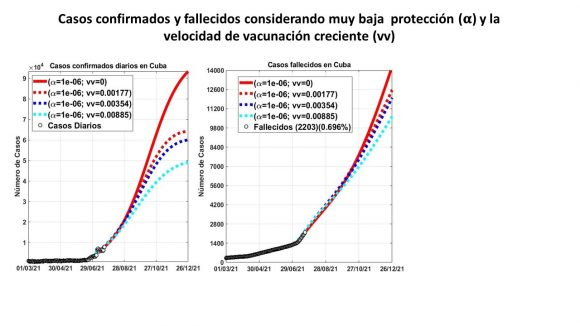
\includegraphics[width=\columnwidth]{cuba debate.jpg}
    \caption{Gráfico de casos comfirmados y fallecidos en el tiempo considerando baja vacunación, fuente: \cite{falcon_reinaldo_arcemontero_izquieroferrer_farinasacostarodriguezmartines_2021}}
    \label{casos cuba debate}
\end{figure}

Para el caso en particular, el Dr. Guinovart Díaz explica, utilizando el modelo anteriormente mencionado, el impacto de la vacunación para Cuba, a mitades del año 2021. Según la figura \ref{casos cuba debate}, al mirar el pronóstico que se genera cuando no se tiene en cuenta una resistencia entregada por la vacuna, es de hasta 9500 casos diarios en un pico. Esto es, considerando que cuba tiene una población de 11.3 millones de habitantes, un caso desastrozo para este país. Cuando se generan esfuerzos vacunativos, estos contagios diarios llegan a un pico de aproximadamente entre 6500 y 5000 casos. Esto aún es desfavorable, pero es una fracción no despreciable respecto a la población sin vacunar.

\begin{figure}
    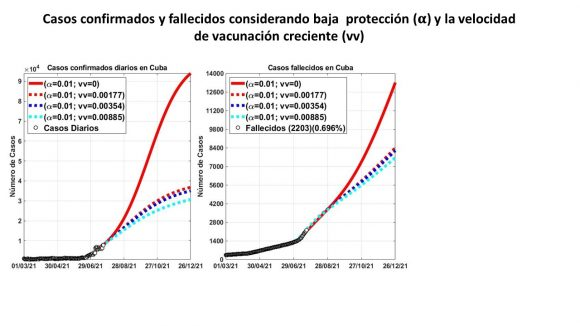
\includegraphics[width=\columnwidth]{cuba debate dos.jpg}
    \caption{Gráfico de casos comfirmados y fallecidos en el tiempo considerando baja vacunación y alto índice de protección, fuente: \cite{falcon_reinaldo_arcemontero_izquieroferrer_farinasacostarodriguezmartines_2021}}
    \label{casos cuba debate dos}
\end{figure}

En una segunda simulación, se hizo el ejercicio similar, pero considerando que solo el 10\% de la población está haciendo el esfuerzo de protegerse, según muestra la figura \ref{casos cuba debate dos}. En este caso, los efectos de la vacuna aumentan aún más drasticamente, y pese a que el pico de casos diarios se mantiene igual para la población sin vacunación, los efectos que demuestra la vacuna en esta simulación es de hasta 1 tercio de lo que resulta en ninguna vacunación.

Aún así se destaca como el gráfico sigue creciendo, e indican ambos que el pico de casos aún está por venir, por lo que la decisión sensata debería ser el aumento del esfuerzo vacunativo, mantener medidas preventivas y de ser posible mejorarlas, y la preparación de los sistemas de salud para la prevención de su colapso conforme llega esta pendiente oleada.
